\documentclass[journal]{IEEEtran}

\usepackage{biblatex}

\usepackage[fleqn]{amsmath}
\usepackage{amssymb}
\usepackage{graphicx}
\usepackage{cancel}
\addbibresource{./citations.bib}

\graphicspath{ {C:/Users/jonat/Documents/ECH-267-Adv.-Proc.-Control/Project/1_Report/images/}}

% \hyphenation{op-tical net-works semi-conduc-tor}


\begin{document}

\title{Nonlinear MPC for Robotic Arm Path Planning and Control \\ ECH-267 Final Project Report}


\author{Jonathan~Dorsey \IEEEmembership{Member: No Sleep Club: est. 2017}}



% The paper headers
\markboth{Journal of Graduate Schooling Assignments, March~2021}%
{Dorsey \MakeLowercase{\textit{et al.}}: Nonlinear MPC for Robotic Arm Path Planning ECH-267 Final Project Report}

% make the title area
\maketitle

% As a general rule, do not put math, special symbols or citations
% in the abstract or keywords.
\begin{abstract}
  The objective of this project is to implement a simulated optimal \underline{Path Planner} using Model Predictive Control (MPC) to plan and control the behavior of a 2 degree of freedom (2DOF) robotic arm. The responsibility of the MPC planner will be to generate the `optimal' path and to drive the arm from its current position to the next. The main challenges faced in completing this project consist of solving for the \textbf{nonlinear equations of motion} (as well as any required forward/inverse kinematics) of the robotic arm as well as formulating and solving the \textbf{MPC controller}, at each timestep, both control and planning using the CasADi optimization framework, to test the scenario of simulated real-time performance.
\end{abstract}

% Note that keywords are not normally used for peerreview papers.
\begin{IEEEkeywords}
Model Predictive Control, Robot Arm, Lagrange Equations, Path Planning, Obsticle Avoidance, DH Parameters, Trajectory Generation.
\end{IEEEkeywords}


\IEEEpeerreviewmaketitle

\section{Introduction}

\IEEEPARstart{T}{he} world of robotics is full of constraints and demands that humans handle naturally and with ease on a daily basis. However, for robotic systems, planning motion or tasks around constraints, limitations, and desired outcomes is a non-trivial task which demands solutions techniques (control and planning) that capable of integrating both hard and soft constraints. Such constraints could manifest across many domains including system performance, physical mobility, design factors, actuation and hardware limitations, to application or task specific processes. One of the many challenges faced in the control design for robotic manipulators conerns how to take all of these constraints into consideration while still performing the assigned tasks. \\

Model Predictive Control (MPC) is an optimal control methodology which solves the a given optimal control problem (OCP) in a receding fashion, over a finite horizon. While these controllers are far more sophisticated than standard classical or modern control strategies, the increased complexity and computation can be applied to a wider class of control problems. \\

One such class of systems are Multiple-Input-Multiple-Output (MIMO), where classical controllers (PID... etc.) become much more involved and less straightforward to utilize effectively. This problem is only exacerbated when the system is nonlinear, which might require techiniques like linearization, feedback-linearization, or gain-scheduling, to effectively control the system using classical or modern control methods. \\

MPC, on the other hand, is a versitile methodology which naturally extends to MIMO systems and seamlessly integrates constraint handling. This flexibility is a property of the underlying structure of the optimal control problem. However, unlike other optimal control solutions such as Linear Quadratic Regulators (LQR), MPC benefits from feedback and thereby increases robustness for modeling or stoichastic uncertainties.  \\

Additionally, MPC can be used to develop an optimal state trajectory or path. This is known as path planning. Due to the predictive nature of MPC, it can not only predict the optimal sequence of inputs, given the current state, it can predict the optimal states required to achieve its objective. By using this ability to predict optimal future states as well as being able to update these predictions required, we can use MPC as a crude path planner. This is often beneficial when direct control of the system is not possible using MPC, but where the planned path can be used as a reference input to the actually controller. \\

This paper will investigate the use of MPC in both planning and control tasks, on a simple robot.


\section{Problem Statement}

The system being used for this project is a two link planar robot arm subject to gravity, as shown in figure (ADD FIGURE). While this robot is simple, it is sufficient to understanding the benefits and draw backs of implementing MPC on a conceptually simple and easily derivable model, unlike more conventional robot manipulators whose dynamics are large and highly coupled.


Instead, this project will utilize a simplified 2-link planar robot which offers many of the same physical challenges a more complex manipulator would but is more suited to be design and test platform for this project, due it relative simplicity.


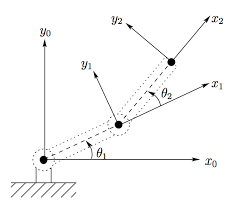
\includegraphics[scale=.5]{2d_arm_2}


As shown in figure (ADD FIGURE NUMBER), the robot itself has two independently actuated links, connected in a serial fashion. Each link is model as a point mass instead of a rigid body for dynamic simplifications.

The overaching objective of this project is to investigate how to use MPC to both control this robot directly, and as a path planner which could be used to supply a reference input to an external controller.




\section{Background}
To discuss the subject of this project in any detail, it is requisite to cover the basic terminology, constructs, and definitions which will be used throughout the remainder of this paper.

\subsection{Robotic Manipulators}

In general robotic arms possess prismatic (linear motion) or revolute (rotational motion) joints. The PUMA 560 robot (INLCUDE FIGURE), is a typical example of an industry standard manipulator, with 6 degrees of freedom (DOF), that utilizes six revolute joints, connected in a serial fashion. This configuration of only rotating joints makes the PUMA 560 an \textbf{articulated robot}. \\

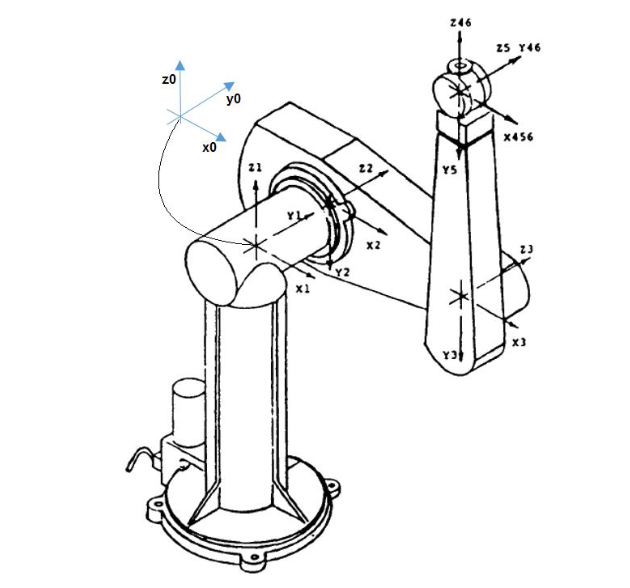
\includegraphics[scale=.5]{puma}

While the study of 6 DOF robots is well researched, the scale and complexity of modeling the governing dynamic equations make robots like the PUMA infeasible for use in this project. Instead, this project will utilize a simplified 2-link planar robot which offers many of the same physical challenges a more complex manipulator would but is more suited to be design and test platform for this project, due it relative simplicity.

\subsection{Trajectory vs Path Generation}

One of the details that often gets overlooked in the difference between a \underline{path} and a \underline{trajectory}. There is, however, a meaningful distinction the two. Paths are independ of time and only consists of a sequence of positions which are meaningful in some way. Trajectories, on the other hand, are dependent on time. This means that for every position in a given trajectory, there is an associated time. This terminology dictates that velocity and acceleration sequences desribe trajectories since both quantities are time dependent. It should be noted that paths can be converted into trajectories by restricting that positions on the path are tracked according to some dependence on time. \\

In the context of this paper, \textbf{path generation} will suffice, since I am only interested in making sure that robotic arm is driven to desired pose (position and orientation) regardless of the time it takes to do so. This is nice simplification to studying and solving trajectory tracking problems and has the nice analytical benefit of making the system dynamics autonomous.

\subsection{Optimal Path Generation}

One interest fact about path planning is that there are infinitely many ways to traverse to two fixed points in continuous space. Therefore one of the engineering challenges is to generate a path with desirable characteristics, for the system being studied. In many cases, it is desirable to obtain the path which defines the shortest distance or time between two points, achievable for a given system. \\

In a broader sense, this means finding the \underline{optimal path} according to some measure of fitness. In the context of robot arm manipulation, the optimal path is that which will direct the robot from an initial pose to a final pose without violating system or path constraints and could even be extended to avoiding obsticles which would otherwise collide with the robot manipulator. \\

% One of the interesting side benefits of using MPC is that we can directly use it to guide the control signal, but we can also use it as a means of online path generation.
%
%
% Being able to generate the optimal state trajectory is a very useful property. Assuming that the objective of the control methodology is actually achieve an optimal path or trajectory can be used as the optimal reference for a variety of other tasks. \\
%
% In this capacity, we can view the MPC system as more or less of an optimal path/trajectory solver; in addition to have the explicity ability to drive the system (as far as physically possible) along this trajectory.
%
%
% Hybrid Control (Supervising Controller)
%
%
%
% While the subjects of model predictive control (MPC) and robotic manipulators (for both design and control), there is exists a lack of targeted literature covering the question about how MPC and robotics can be used in the domain of real-time path planning.
%
%
%   It has long be known that MPC is viable controller with many flavors and versions for different applications; however, in practice MPC only sees limited use due to the computational lag resulting from using numerical optimization as the basis for feedback control.
%
%   To this end, MPC might be too slow for use in the control of a system, but if the optimal trajectory can be estimated using MPC, other controllers might be better suited for the task of tracking the optimal path which the MPC controller is able to generate.
%
%   Since this path is only updated as needed, the speed of the MPC solution is no longer a significant obsticle since we can effectively offload the task of controller to a less computationally expensive methodology.

\subsection{Model Predictive Control}

As previously illuded to, MPC is an optimization based controller that solves for the



\subsection{Path Planner}

\subsection{Articulated Robotic Systems}



\subsubsection{Governing Equations for Serial Robots}







\subsubsection{Denavit-Hartenberg Paramters}
The Denavit-Hartenberg (DH) parameters are an important tool in analyzing the geometry of any given robot as well as in the formulation of joint transformations which enable a concise and universal means of deriving important quanties for kinematic and dynamic analysis of the robot.

The purpose of DH parameters is to standardize the description of geometry of robots into a universal parameterization such that arbitary construction of different robots can all be described concisely in a single and intuitive notation. \\

\noindent The DH Parameters are defined to be...
$$
\begin{array}{l}
a_{i}=\text { the distance from } \hat{Z}_{i} \text { to } \hat{Z}_{i+1} \text { measured along } \hat{X}_{i} \\
\alpha_{i}=\text { the angle from } \hat{Z}_{i} \text { to } \hat{Z}_{i+1} \text { measured about } \hat{X}_{i} \\
d_{i}=\text { the distance from } \hat{X}_{i-1} \text { to } \hat{X}_{i} \text { measured along } \hat{Z}_{i} ; \text { and } \\
\theta_{i}=\text { the angle from } \hat{X}_{i-1} \text { to } \hat{X}_{i} \text { measured about } \hat{Z}_{i}
\end{array}
$$

The primary usage of DH Parameters is the generation of transformations to and from joint frame origins. Before this can be achieved, there needs to exist the notion of a general transformation which captures both position and orientation (e.g. pose) from one frame to another. By coupling position vectors to the origin of each joint frame and the corresponding rotation matrix, we arrive at the following \textbf{homogeneous transforms}.


$$
\left[\begin{array}{c}
{}^{A}P \\
1
\end{array}\right]=\left[\begin{array}{ccc|c}
{} & {}^{A}_{B}R & & {}^{A}P_{B org} \\
\hline 0 & 0 & 0 & 1
\end{array}\right]\left[\begin{array}{c}
{}^{B}P \\
1
\end{array}\right]
$$



Which can be further simplified to...

$$
P={ }_{B}^{A} T^{B} P
$$

Since the DH Parameters provide a universal notation for describing the the position and orientation of a robot, it is natural to want to express the homogeneous transformation of each coordinate frame using this parameterization. For a single transformation from a frame $\{ i\}$ to frame $\{ i-1 \}$, we can use the homogeneous transformation for explicit rotations about a joint axis or specific translations along a joint axis as dictated by the DH parameters.The matrices $R$ and $D$ represent the homogeneous transformation for rotation and translations repsectively, with the subscript of each providing the axis upon which the operation should be performed.

$$
{ }_{i}^{i-1} T=R_{X}\left(\alpha_{i-1}\right) D_{X}\left(a_{i-1}\right) R_{Z}\left(\theta_{i}\right) D_{Z}\left(d_{i}\right)
$$


By using the universal, DH paramterization with homogeneous transformation we can now describe the relationships to or from any joint of the robot to any other joint of the robot. This is a powerful concept which facilitates the analysis of any robot whose joints are based on revolute or prismatic members.





\subsubsection{Forward Kinematics}
Forward Kinematics (FK) is the study how the final pose of a manipulator given joint positions and velocities. By using DH parameter based transformations, the position or velocity of any joint can computed against the given frame of refernce (often the {0} frame).


\subsubsection{Inverse Kinematics}

Inverse Kinematics (IK) is the study of the joint positions and velocities given the position and velocity of the manipulator. IK is typically a harder task to perform than FK since there are often multiple solutions which satisfy the pose of the end effector.


\subsubsection{Forward Dynamics}



\subsubsection{Inverse Dynamics}





\section{MPC Formulation}

The mathematical basis for MPC stems from the standard optimal control problem. However, with a few slight adjustments and relaxations, the formulation for MPC can be


\subsection{MPC Assumptions}

\begin{enumerate}
  \item Internal dynamic model of system exists
  \item Finite (and receding) prediction horizion
  \item Piecewise constant input at each time-step \\
\end{enumerate}

After applying these restrictions to the standard optimal control problem, the mathematical formulation for standard MPC reduces to the following expression.

\begin{equation}
\begin{aligned}
& \min _{n} J_{x}\left(\mathbf{x}_{0}, \mathbf{u}\right)=\sum_{k=0}^{N-1} \ell\left(\mathbf{x}_{\mathbf{v}}(k), \mathbf{u}(k)\right) \\
\text { s.t: }: & \mathbf{x}_{\mathbf{n}}(k+1)=\mathbf{f}\left(\mathbf{x}_{\mathbf{n}}(k), \mathbf{u}(k)\right) \\
& \mathbf{x}_{\mathbf{u}}(0)=\mathbf{x}_{0}, \\
& \mathbf{u}(k) \in U, \forall k \in[0, N-1] \\
& \mathbf{x}_{\mathbf{u}}(k) \in X, \forall k \in[0, N]
\end{aligned}
\end{equation}

In this formulation, the cost function is only propagated to the end of the prediction horizon $N$, from the current initial state of the system. The first equality constraint restricts future states of the system to be feasible with respect to the system model. The second equality constraints requires the initial state of the solver to be the current initial state of the system, while the final constraints require the inputs and states determined by the solver to be valid elements of feasible input and state sets respectively. \\


The particular flavor of MPC used in this project utilized the following quadratic stage cost.

\begin{equation}
  \ell\left(\mathbf{x}_{\mathbf{v}}(k), \mathbf{u}(k)\right) = (x-x_d)Q(x-x_d) + (u-u_d)R(u-u_d)
\end{equation}

This parameterization stage cost can be further simplified using norms.


\begin{equation}
  \ell\left(\mathbf{x}_{\mathbf{v}}(k), \mathbf{u}(k)\right) = \left\Vert x - x_d \right\Vert^{2}_{Q} + \left\Vert u -u_d \right\Vert^{2}_{R}
\end{equation}

The quadratic nature of this cost function is eligant in how simple and intuitive it is comprehend as as well how simple it is to tune using the matrices $Q$ and $R$. \\

It should be further noted that this project uses the \textbf{Multiple Shooting} implementation of MPC as this approach has shown to produce better results and obtained solutions far faster than the naive single shooting approach.




\section{Path Planner}

An addition benefit to using multiple shooting is that since the state predictions over the time horizon are included as decision variables along with the input sequence, the very produce of solving for the optimal inputs (over the prediction horizon) also yields the predicted states without necessitating forward propigating the optimal input and current state through the system model.\\

Because of this fact, at any given instance, the MPC controller not only yields the optimal inputs, but specifies the optimal state trajectory over the prediction horizion. \\

By leveraging this fact, we can fit a cubic spline through those discrete state predictions. Once calculated, this spline can be used to as a refernce path to calculate reference joint positions for a controller to track. \\

Naturally, as the prediction horizon used for MPC probably does not span the entire path required to drive the robot from its initial pose to its desired pose, the reference path will be need to be recomputed occationally, if the predictions from the model deviate from the actual measurements of the system (or state estimator outputs).



\section{Dynamics Model}

For this project, the model of the robot will only include the dynamics of the physical system and not the dynamics of the actuators. However, it would be trivial to include these effects for a more realistic model of how the system operates, but for the purposes of simplicity, we will assume that the joint motors have perfect torque control. \\

A further simplification to modeling this system is that we assume massless links and that each point can be modeled as a point mass. Under these assumptions, we can ignore contributions by moments of inertia. This simplifies the process of deriving equations of motion. \\

The method to derive the dynamics of the modeled system uses the \textbf{Euler-Lagrange Equations}. This is variational method which uses the kinetic and potential energies of the system to derive the dynamics of the robot. While equivalent to the Newton-Euler Equations, Lagrange Equations do not require the computing of accelerations and typically simplify the derivation of

\begin{equation}
k_{i}=\frac{1}{2} m_{i} v_{C_{i}}^{T} v_{C_{i}}+\frac{1}{2}^{i} \omega_{i}^{T} C_{i} I_{i}^{i} \omega_{i}
\end{equation}


\begin{equation}
u_{i}=-m_{i}^{0} g^{T}{ }^{0} P_{C_{i}}+u_{r e f_{i}}
\end{equation}

\begin{equation}
k=\sum_{i=1}^{n} k_{i}
\end{equation}

\begin{equation}
u=\sum_{i=1}^{n} u_{i}
\end{equation}

\begin{equation}
  L = k - u
\end{equation}

\begin{equation}
\frac{d}{d t} \frac{\partial L}{\partial \dot{\boldsymbol{q}}}-\frac{\partial L}{\partial \boldsymbol{q}}=\left[\begin{array}{l}
\tau_{1} \\
\tau_{2}
\end{array}\right]
\end{equation}


\subsection{Nonlinear Model}
In general, the serially articulated robots with revolute joints will produce equations of motion (EOM) that take the following form.

\begin{equation}
  \tau = M(\Theta)\ddot{\Theta} + V(\Theta, \dot{\Theta}) + G(\Theta) + F(\dot{\Theta})
\end{equation}


In this formulation, $M$ is the mass matrix which models the effects of mass and moments of inertia which are related to the angular accelerations of the joints. The $V$ vector models the centrifugal and Coriolis forces which are typically functions of velocities, while the $G$ vector models the effects of gravity. Finally, the $F$ vector is added to explictly include the effects of friction/damping.

\begin{equation}
\begin{aligned}
M(\theta)=\left[\begin{array}{ll}
 m_{11} & m_{12}  \\
 m_{21} & m_{22} \end{array}\right]
\end{aligned}
\end{equation}

Where

\begin{equation*}
\begin{aligned}
  m_{11} & = m_{1} L_{1}^{2}+m_{2}\left(L_{1}^{2}+2 L_{1} L_{2} \cos \left(\theta_{1}\right)+L_{2}^{2}\right) + \varepsilon \\
  m_{12} & = m_{2}\left(L_{1} L_{2} \cos \left(\theta_{2}\right)+L_{2}^{2}\right) \\
  m_{21} & = m_{2}\left(L_{1} L_{2} \cos \left(\theta_{2}\right)+L_{2}^{2}\right)\\
  m_{22} & = m_{2} L_{2}^{2}+\varepsilon
\end{aligned}
\end{equation*}



\begin{equation}
V(\theta, \dot{\theta})=\left[\begin{array}{c}
-m_{2} L_{1} L_{2} \sin \left(\theta_{2}\right)\left(2 \dot{\theta}_{1} \dot{\theta}_{2}+\dot{\theta}_{2}^{2}\right) \\
m_{2} L_{1} L_{2} \dot{\theta}_{1}^{2} \sin \left(\theta_{2}\right)
\end{array}\right]
\end{equation}


\begin{equation}
G(\theta)=\left[\begin{array}{c}
\left(m_{1}+m_{2}\right) L_{1} g \cos \left(\theta_{1}\right)+m_{2} g_{2} \cos \left(\theta_{1}+\theta_{2}\right) \\
m_{2} g L_{2} \cos \left(\theta_{1}+\theta_{2}\right)
\end{array}\right]
\end{equation}


\begin{equation}
F(\dot{\theta})=\left[\begin{array}{c}
c_{f} \cdot \dot{\theta}_{1} \\
c_{f} \cdot \dot{\theta}_{2}
\end{array}\right]
\end{equation}


It should be noted for simulation purposes, the equations of motion need to express $\tau$ as the input to the robot and the angular accelerations $\ddot{\Theta}$ as the outputs.

\begin{equation}
\ddot{\theta}=\operatorname{inv}(M)[\tau-V-G-F]
\end{equation}

However, expressing the governing equations in this form result in numerical instabilties during simulation which arise from inverting the mass matrix $M(\Theta)$. Since the mass matrix is function if the angular positions $\Theta$, certain angular positions will cause the mass matrix to near a singularity, when inverted, at which the numerical values explode until they become \textbf{INF} or \textbf{NAN}. To avoid this, the value of $\varepsilon$ can be added to the diagonal terms of $M$ to garuntee that the system will never become singular, during inversion.


With equation (EQN NUMBER), we can now write the equivalent nonlinear state space for the system. By defining the states such that, $x_{1}=\theta_{1}$, $x_{2}=\theta_{2}$, $x_{3}=\dot{\theta}_{1}$, and $x_{4}=\dot{\theta}_{2}$, we can


\begin{equation}
\begin{array}{l}
\dot{x}_{1}=f_{1}(x, \dot{x}, u) \\
\dot{x}_{2}=f_{2}(x, \dot{x}, u) \\
\dot{x}_{3}=f_{3}(x, \dot{x}, u) \\
\dot{x}_{4}=f_{4}(x, \dot{x}, u)
\end{array}
\end{equation}


Such that


\begin{equation}
\begin{array}{l}
\dot{x}_{1}=x_{3} \\
\dot{x}_{2}=x_{4} \\
\dot{x}_{3}=\ddot{\theta}_{1} \\
\dot{x}_{4}=\ddot{\theta}_{2}
\end{array}
\end{equation}




\begin{equation}
\begin{array}{l}
\dot{x}_{1}=x_{3} \\
\dot{x}_{2}=x_{4} \\
\dot{x}_{3}=\frac{5\,\left(10\,{L_{2}}^2\,m_{2}\,q_{\dot{2}}-10\,{L_{2}}^2\,m_{2}\,q_{\dot{1}}-q_{\dot{1}}-4\,L_{2}\,g\,m_{2}\,\cos\left(q_{1}+q_{2}\right)-4\,L_{1}\,g\,m_{1}\,\cos\left(q_{1}\right)-4\,L_{1}\,g\,m_{2}\,\cos\left(q_{1}\right)+4\,L_{1}\,L_{2}\,m_{2}\,{q_{\dot{2}}}^2\,\sin\left(q_{2}\right)-40\,L_{1}\,{L_{2}}^2\,g\,{m_{2}}^2\,\cos\left(q_{1}\right)+20\,{L_{1}}^2\,{L_{2}}^2\,{m_{2}}^2\,{q_{\dot{1}}}^2\,\sin\left(2\,q_{2}\right)+10\,L_{1}\,L_{2}\,m_{2}\,q_{\dot{2}}\,\cos\left(q_{2}\right)+40\,L_{1}\,{L_{2}}^3\,{m_{2}}^2\,{q_{\dot{1}}}^2\,\sin\left(q_{2}\right)+40\,L_{1}\,{L_{2}}^3\,{m_{2}}^2\,{q_{\dot{2}}}^2\,\sin\left(q_{2}\right)+40\,L_{1}\,{L_{2}}^2\,g\,{m_{2}}^2\,\cos\left(q_{1}+q_{2}\right)\,\cos\left(q_{2}\right)+8\,L_{1}\,L_{2}\,m_{2}\,q_{\dot{1}}\,q_{\dot{2}}\,\sin\left(q_{2}\right)-40\,L_{1}\,{L_{2}}^2\,g\,m_{1}\,m_{2}\,\cos\left(q_{1}\right)+80\,L_{1}\,{L_{2}}^3\,{m_{2}}^2\,q_{\dot{1}}\,q_{\dot{2}}\,\sin\left(q_{2}\right)\right)}{2\,\left(-100\,{L_{1}}^2\,{L_{2}}^2\,{m_{2}}^2\,{\cos\left(q_{2}\right)}^2+100\,{L_{1}}^2\,{L_{2}}^2\,{m_{2}}^2+100\,m_{1}\,{L_{1}}^2\,{L_{2}}^2\,m_{2}+10\,{L_{1}}^2\,m_{2}+10\,m_{1}\,{L_{1}}^2+20\,L_{1}\,L_{2}\,m_{2}\,\cos\left(q_{2}\right)+20\,{L_{2}}^2\,m_{2}+1\right)} \\
\dot{x}_{4}=-\frac{5\,\left(q_{\dot{2}}+10\,{L_{1}}^2\,m_{1}\,q_{\dot{2}}+10\,{L_{1}}^2\,m_{2}\,q_{\dot{2}}-10\,{L_{2}}^2\,m_{2}\,q_{\dot{1}}+10\,{L_{2}}^2\,m_{2}\,q_{\dot{2}}+4\,L_{1}\,L_{2}\,m_{2}\,{q_{\dot{1}}}^2\,\sin\left(q_{2}\right)+4\,L_{2}\,g\,m_{2}\,\cos\left(q_{1}\right)\,\cos\left(q_{2}\right)-4\,L_{2}\,g\,m_{2}\,\sin\left(q_{1}\right)\,\sin\left(q_{2}\right)-20\,L_{1}\,{L_{2}}^2\,g\,{m_{2}}^2\,\cos\left(q_{1}\right)+40\,{L_{1}}^2\,{L_{2}}^2\,{m_{2}}^2\,{q_{\dot{1}}}^2\,\sin\left(2\,q_{2}\right)+20\,{L_{1}}^2\,{L_{2}}^2\,{m_{2}}^2\,{q_{\dot{2}}}^2\,\sin\left(2\,q_{2}\right)-10\,L_{1}\,L_{2}\,m_{2}\,q_{\dot{1}}\,\cos\left(q_{2}\right)+20\,L_{1}\,L_{2}\,m_{2}\,q_{\dot{2}}\,\cos\left(q_{2}\right)+40\,L_{1}\,{L_{2}}^3\,{m_{2}}^2\,{q_{\dot{1}}}^2\,\sin\left(q_{2}\right)+40\,{L_{1}}^3\,L_{2}\,{m_{2}}^2\,{q_{\dot{1}}}^2\,\sin\left(q_{2}\right)+40\,L_{1}\,{L_{2}}^3\,{m_{2}}^2\,{q_{\dot{2}}}^2\,\sin\left(q_{2}\right)-40\,{L_{1}}^2\,L_{2}\,g\,{m_{2}}^2\,\sin\left(q_{1}\right)\,\sin\left(q_{2}\right)-40\,L_{1}\,{L_{2}}^2\,g\,m_{1}\,m_{2}\,\cos\left(q_{1}\right)+20\,L_{1}\,{L_{2}}^2\,g\,{m_{2}}^2\,\cos\left(2\,q_{2}\right)\,\cos\left(q_{1}\right)+40\,{L_{1}}^2\,{L_{2}}^2\,{m_{2}}^2\,q_{\dot{1}}\,q_{\dot{2}}\,\sin\left(2\,q_{2}\right)-20\,L_{1}\,{L_{2}}^2\,g\,{m_{2}}^2\,\sin\left(2\,q_{2}\right)\,\sin\left(q_{1}\right)+40\,{L_{1}}^3\,L_{2}\,m_{1}\,m_{2}\,{q_{\dot{1}}}^2\,\sin\left(q_{2}\right)+80\,L_{1}\,{L_{2}}^3\,{m_{2}}^2\,q_{\dot{1}}\,q_{\dot{2}}\,\sin\left(q_{2}\right)-40\,{L_{1}}^2\,L_{2}\,g\,m_{1}\,m_{2}\,\sin\left(q_{1}\right)\,\sin\left(q_{2}\right)\right)}{2\,\left(-100\,{L_{1}}^2\,{L_{2}}^2\,{m_{2}}^2\,{\cos\left(q_{2}\right)}^2+100\,{L_{1}}^2\,{L_{2}}^2\,{m_{2}}^2+100\,m_{1}\,{L_{1}}^2\,{L_{2}}^2\,m_{2}+10\,{L_{1}}^2\,m_{2}+10\,m_{1}\,{L_{1}}^2+20\,L_{1}\,L_{2}\,m_{2}\,\cos\left(q_{2}\right)+20\,{L_{2}}^2\,m_{2}+1\right)}
\end{array}
\end{equation}











Linearizing the system required computing the Jacobian of the nonlinear state space, and evaluating the resulting matrix at specified equilibrium points, such that around a small neighborhood the system will behavior linearly.



\subsection{Obsticle Avoidance}


\section{Results}

\subsection{Direct Control via MPC}

From a purely controls perspective, MPC performed quite well. The nonlinear nature of the system made would have made required simplifications to the system model to be made before a

\includegraphics[scale = 0.5]{../images/Nominal_MPC/T1_X_init_25_45_0_0_X_ref_180_n45_0_0/Torques}


\includegraphics[scale = 0.5]{../images/Nominal_MPC/T1_X_init_25_45_0_0_X_ref_180_n45_0_0/AngularPositions}


\includegraphics[scale = 0.5]{../images/Nominal_MPC/T1_X_init_25_45_0_0_X_ref_180_n45_0_0/AngularVelocities}




\includegraphics[scale = 0.5]{../images/Nominal_MPC/T4_X_init_220_25_0_0_X_ref_180_n45_0_0/Torques}


\includegraphics[scale = 0.5]{../images/Nominal_MPC/T4_X_init_220_25_0_0_X_ref_180_n45_0_0/AngularPositions}


\includegraphics[scale = 0.5]{../images/Nominal_MPC/T4_X_init_220_25_0_0_X_ref_180_n45_0_0/AngularVelocities}





\subsection{Model/System Mismatch}

\subsection{}

\subsection{}

\subsection{}

\subsection{}

\subsection{}

\subsection{}

\subsection{}

\section{Discussion}

Dicussion and points of note.


\subsection{Direct Control via MPC}

In general, control of the robot using MPC was very successful. In each ``pose-to-pose" test performed, MPC was able to drive the system from its initial state to the final state within 4 decimals of precision In addition to achieving the stated objective, MPC was able to keep the able to handle the limits of the actuators even

Since this robot is subject to gravity,

\subsection{MPC with System Constraints}

One interested test case for directly using MPC to control the robot is the situatation where there exist physical limits on the rotation of the each link, that prevents the robot from being able to actuate beyond a certain range. In this case, it is desireable to for the controller to recognize these limitations and find the best possible path to get to the goal position.





Additionally, it was interesting to see how MPC performed when the goal state was infeasible by virtue of physical constraints of the robot. In such a case, I found that while the controller did not ever violate the constraints, it would drive the robot into an apparently random pose.


\subsection{Path Planning via MPC}

While definitely able to generate paths using MPC, path planning was significantly more challenging than anticipated. I be



\section{Conclusion}
The conclusion goes here.


% \appendices
% \section{Proof of the First Zonklar Equation}
% Appendix one text goes here.
%
%
% \section{}
% Appendix two text goes here.


\section*{Acknowledgment}


The authors would like to thank Mountain Dew and his matress for constant support and comfort.



\ifCLASSOPTIONcaptionsoff
  \newpage
\fi



% \begin{thebibliography}{1}
%
% \bibitem{IEEEhowto:kopka}
% H.~Kopka and P.~W. Daly, \emph{A Guide to \LaTeX}, 3rd~ed.\hskip 1em plus
%   0.5em minus 0.4em\relax Harlow, England: Addison-Wesley, 1999.
%
%       \bibitem{}  J. B. Rawlings, M. M. Diehl, and D. Q. Mayne, Model predictive control: theory, computation and design. Madison: Nob Hill, 2017.
%
%       \bibitem{} B. Armstrong, O. Khatib and J. Burdick, "The explicit dynamic model and inertial parameters of the PUMA 560 arm," Proceedings. 1986 IEEE International Conference on Robotics and Automation, San Francisco, CA, USA, 1986, pp. 510-518, doi: 10.1109/ROBOT.1986.1087644.
%
% \end{thebibliography}
\cite{craig_introduction_2005}
\cite{khalil_nonlinear_2002}
\cite{rawlings_model_2017}
\cite{armstrong_explicit_1986}
\cite{ogata_modern_2010}
\cite{meriam_engineering_1993}
\cite{greenwood_advanced_2006}
\cite{borrelli_predictive_2017}
\cite{boyd_convex_2004}
\cite{slotine_applied_1991}
\cite{soft_constraints}

\printbibliography

\begin{IEEEbiography}[{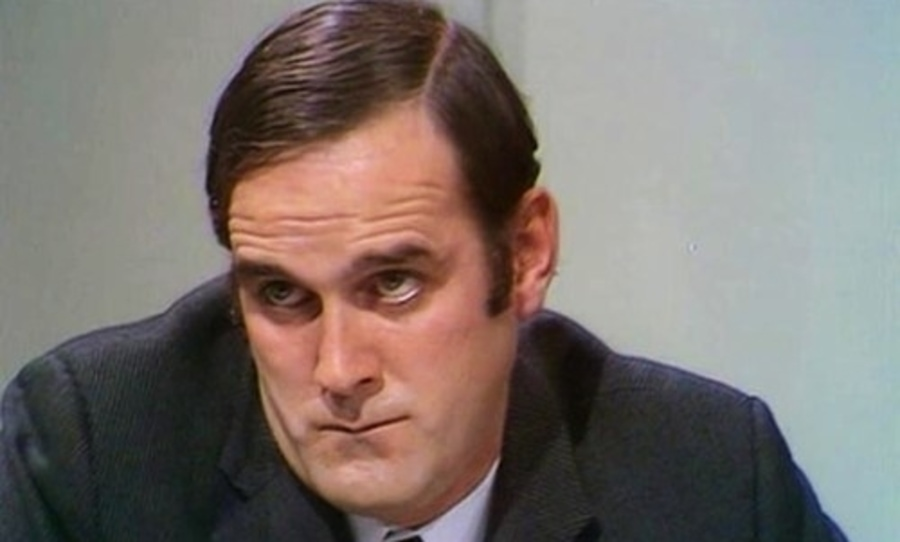
\includegraphics[width=1in,height=1.25in,clip,keepaspectratio]{monty1}}]{Jonathan Dorsey}
  I've already told you once. It is an ex parrot. Its has ceased to be. Recieved his Bachelors Degree in Mechanical Engineering from the San Jose State University. With a focus on mechatronics and control systems, he has developed an interest in reinforcement learning, computer vision, and control and design of autonomous systems.
\end{IEEEbiography}



\end{document}
